% #############################################################################
% This is Chapter 1
% !TEX root = ../main.tex
% #############################################################################
% Change the Name of the Chapter i the following line
\fancychapter{Introduction}
\cleardoublepage
% The following line allows to ref this chapter
\label{chap:intro}
Referring expression segmentation is a computer vision task in which a model receives a natural language description of a target region and must return the corresponding segmentation mask. Because the phrasing can reference any concept, the task is open-vocabulary and the target can be a single instance, a coherent group of instances, or an entire semantic category, such as "all roads in the patch" or "the vegetation strip along the river". The remote-sensing literature coined the term Referring Remote Sensing Instance Segmentation (RRSIS)~\cite{yuan2023rrsis} for the subset that limits expressions to single instances, while later datasets like NWPU-Refer~\cite{yang2024large} incorporated group-level expressions, and Aerial-D extends the coverage further to include instances, groups, and full land-cover classes. When this formulation is applied to aerial photographs, although we refer to it simply as referring expression segmentation throughout this thesis, the problem becomes especially demanding because top-down perspectives compress object scales, spatial resolution varies across sensors, many targets occupy only a handful of pixels, and the scenes themselves contain extreme object densities. In many real deployments, analysts revisit archival aerial surveys to study how cities or coastlines evolved. To support that use case, the pipeline also models the monochrome, sepia, and grainy degradations found in historic imagery so the resulting models can handle tasks such as assessing long-term urban change.

A critical component for developing effective models for RRSIS and broader referring segmentation of aerial photographs is access to high-quality datasets containing aerial imagery, precise segmentation masks, and natural referring expressions. To address this need, this work presents Aerial-D, a large-scale referring expression segmentation dataset for aerial imagery comprising 1,522,523 expressions across 37,288 aerial image patches, significantly larger than prior RRSIS benchmarks~\cite{yuan2023rrsis,liu2024rotated,yang2024large}. Figure~\ref{fig:dataset_examples_intro} highlights how this corpus spans rural and urban scenes and objects, land-cover regions, groups of multiple objects, and entire categories while retaining unrestricted, richly worded referring expressions tailored to each target.

\begin{figure}[t]
\centering
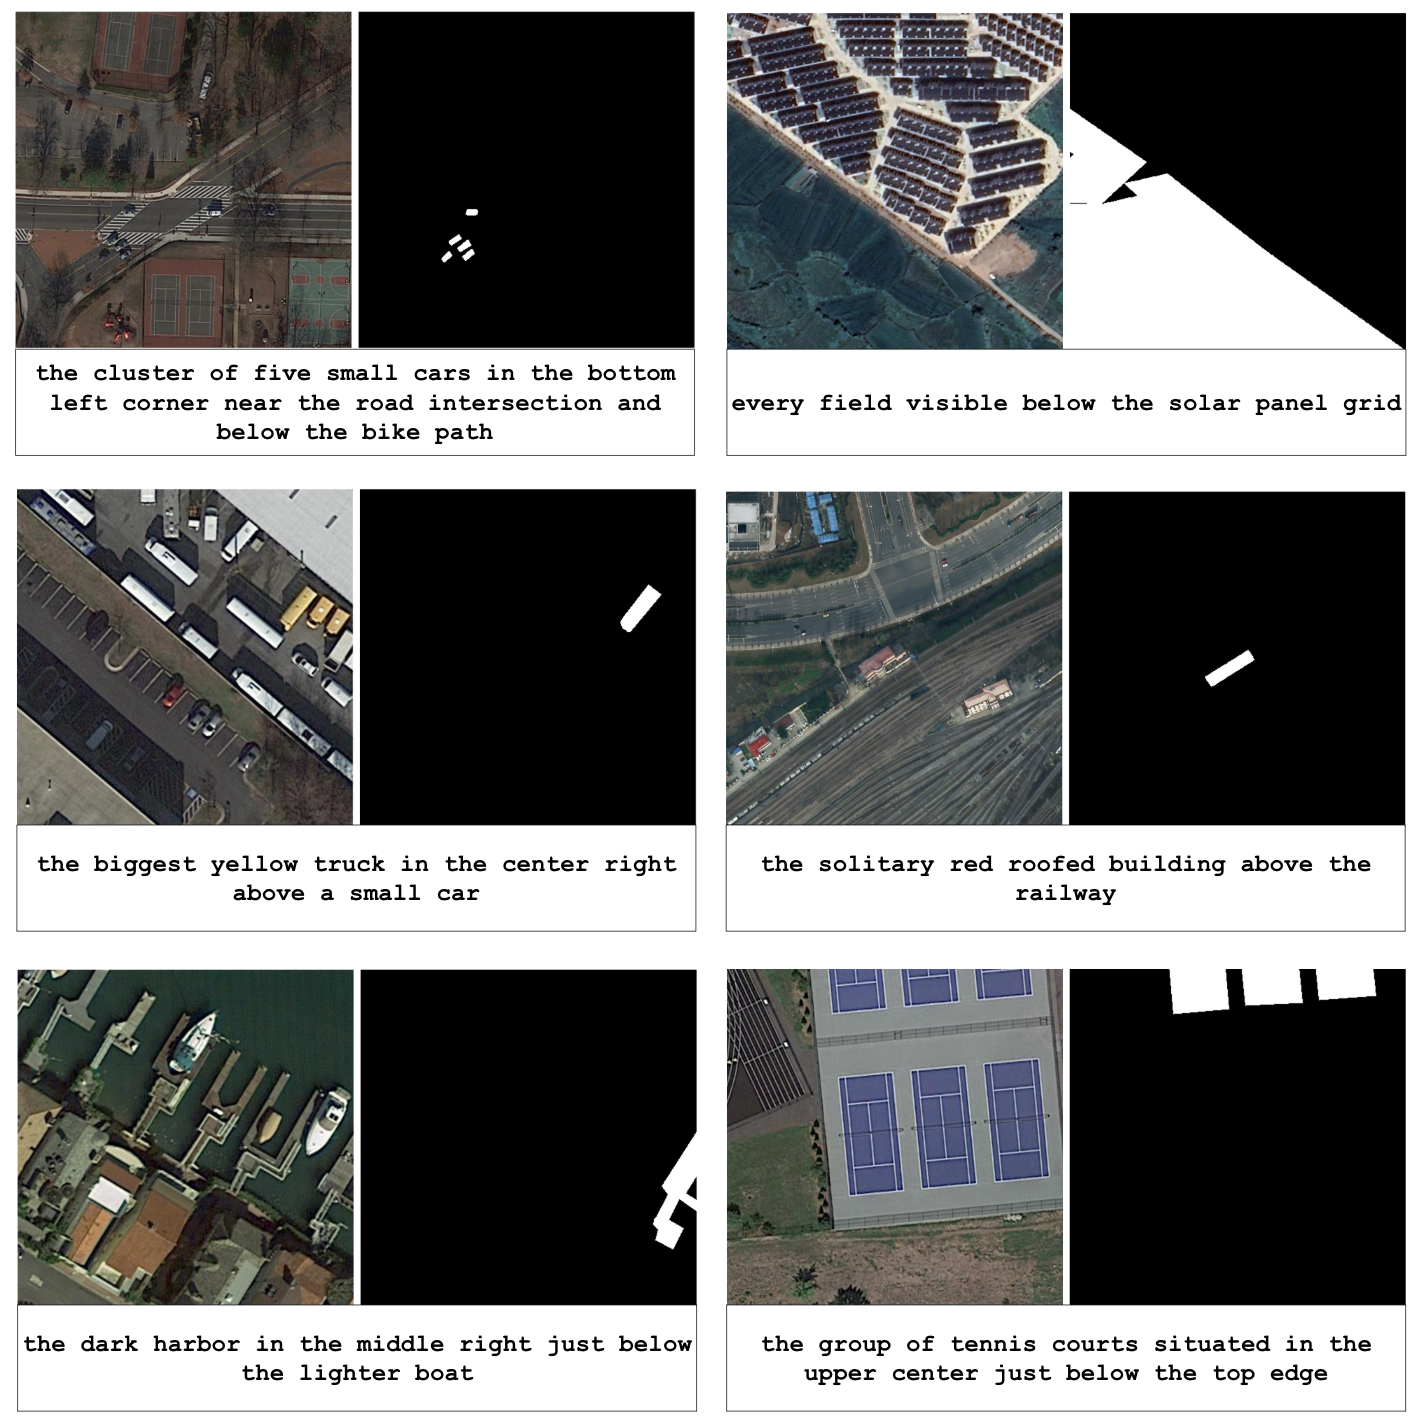
\includegraphics[width=\textwidth]{Images/6samples.png}
\caption{Representative examples from Aerial-D dataset showing diverse referring expressions with corresponding aerial images and ground truth masks.}
\label{fig:dataset_examples_intro}
\end{figure}

% #############################################################################
\section{Contributions}

The key contributions of this work include: (1) a comprehensive toolchain that enables the production of complex referring expression datasets from instance/semantic segmentation datasets, including a rule-based pipeline, Large Language Model enhancement and distillation methods, and historic image data augmentation with dedicated filtering; (2) the construction of Aerial-D, a dataset comprising over 1.5 million expressions across 37,288 aerial image patches, created entirely through the proposed automatic pipeline; and (3) a unified model trained on Aerial-D alongside four additional datasets, leveraging historic transformations and other applicable components of the toolchain across the training data to deliver referring expression segmentation over instances, groups, classes, and land cover regions while maintaining reliable performance on degraded historic imagery typical of archival aerial surveys.
% #############################################################################
\section{Document Structure}

This thesis is organized into six chapters and one appendix, each addressing distinct aspects of the methodology and evaluation:

\textbf{Chapter 2: Fundamental Concepts} establishes the theoretical foundation by introducing neural networks and deep learning principles, transformer architectures, computer vision fundamentals for image segmentation, and vision-language models. This chapter covers essential background on CLIP models, large language models, and the intersection of computer vision and natural language processing that enables referring segmentation.

\textbf{Chapter 3: Related Work} provides a comprehensive review of existing research in aerial image segmentation datasets, ranging from traditional semantic and instance segmentation datasets to specialized referring segmentation benchmarks. The chapter examines vision backbones for segmentation tasks, state-of-the-art referring segmentation models, and the emerging application of large language models to computer vision problems.

\textbf{Chapter 4: Aerial-D Dataset Construction} presents the systematic methodology for constructing the Aerial-D dataset. The chapter details the source datasets (iSAID~\cite{zamir2019isaid} and LoveDA~\cite{wang2021loveda}), the rule-based expression generation pipeline that transforms instance and semantic masks into referring expressions, LLM-based enhancement techniques using Gemma3, model distillation approaches, and comprehensive dataset statistics demonstrating the scale and diversity of the final resource.

\textbf{Chapter 5: Experiments} describes the experimental evaluation of the proposed approach using the RSRefSeg model architecture. The chapter covers the model implementation details, experimental setup across multiple benchmarks, comprehensive results on Aerial-D and comparison datasets including RRSIS-D, NWPU-Refer, RefSegRS, and Urban1960SatSeg, and ablation studies analyzing the contribution of different dataset enhancement components.

\textbf{Chapter 6: Conclusion and Future Work} synthesizes the key findings and contributions of this research while identifying promising directions for future investigation. The chapter summarizes the effectiveness of the automated dataset generation approach, discusses the implications for aerial image analysis, and outlines potential extensions to other remote sensing applications.

\textbf{Appendix A: LLM Enhancement Prompt} contains the complete system and user prompts employed during the Gemma3-based enhancement phase of dataset construction, providing full transparency and reproducibility for the LLM annotation process.